\subsection{Face Recognition dengan kamera}
\begin{enumerate}
    \item Proses pengumpulan dataset
    
    - Memasukan library openCV \textbf{cv2} serta \textbf{os}. Librari \textbf{os}
    digunakan untuk mengakses fungsi pada sistem operasi
    \begin{figure}[h!]
        \centering
        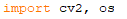
\includegraphics[width=0.3\linewidth]{images/fr_cam1.PNG}
        \caption{Memasukan library }
    \end{figure}

    - Proses face detection dengan memasukan algoritma \emph{haar-cascade classifier} serta
     memasukan video dengan \textbf{cv2.VideoCapture()}
     \begin{figure}[h!]
        \centering
        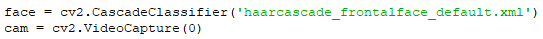
\includegraphics[width=0.9\linewidth]{images/fr_cam2.PNG}
        \caption{Proses face detection dengan masukan kamera}
    \end{figure}

    - Membuat inputan untuk id serta label folder pada kumpulan dataset, pembuatan folder label dataset menggunakan 
    library \textbf{os} yang menggunakan fungsi sitem operasi \textbf{mkdir}
    \begin{figure}[h!]
        \centering
        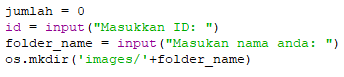
\includegraphics[width=0.7\linewidth]{images/fr_cam3.PNG}
        \caption{Masukan id serta nama untuk label dataset}
    \end{figure}

    - Proses deteksi wajah dan pengambilan dataset sebanyak 40 sample yang dimasukan pada direktori label
    \begin{figure}[h!]
        \centering
        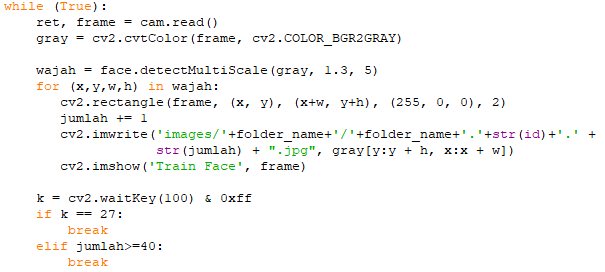
\includegraphics[width=0.9\linewidth]{images/fr_cam4.PNG}
        \caption{Proses face detection dan pengambilan dataset}
    \end{figure}

    - Hasil pengambilan dataset
    \begin{figure}[h!]
        \centering
        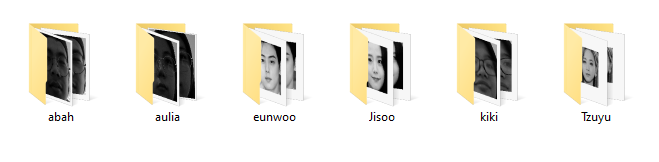
\includegraphics[width=1\linewidth]{images/fr_cam5.PNG}
        \caption{Kumpulan label direktori dataset}
        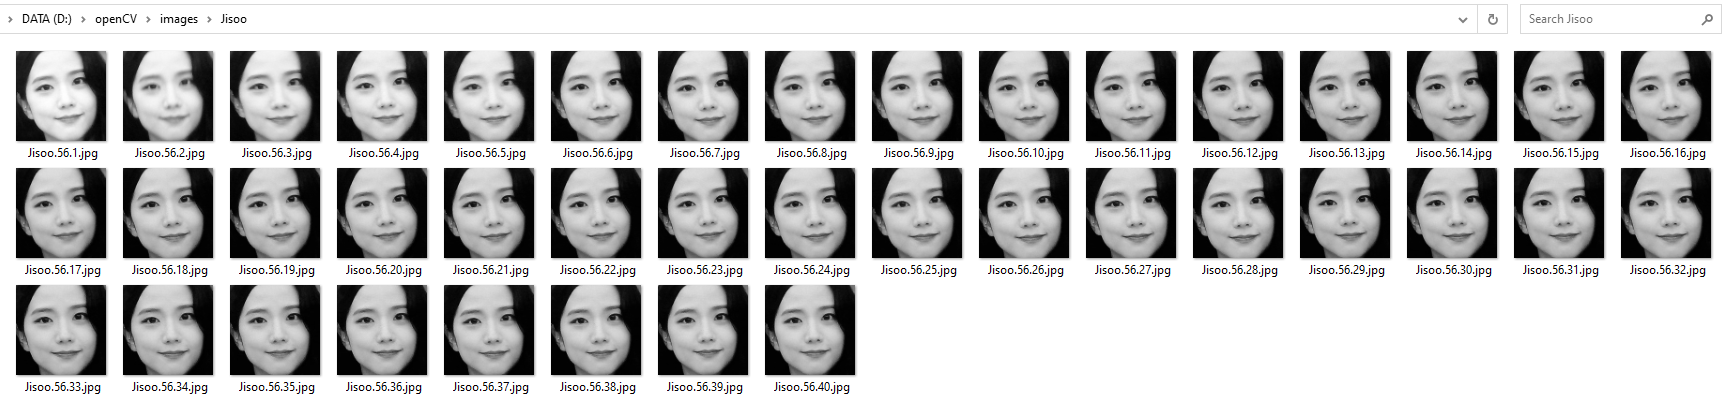
\includegraphics[width=1.1\linewidth]{images/fr_cam6.PNG}
        \caption{Isi direktori salah satu label dataset}
    \end{figure}
    \item Proses training dataset
    
    - Import library, training dataset kali ini memerlukan library baru yaitu : 
    \begin{enumerate}[*]
        \item \textbf{os} untuk mengakses fungsi pada sistem operasi,
        \item \textbf{pickle} untuk menyimpan dan membaca data ke dalam/dari sebuah file, dan
        \item \textbf{Image dari PIL} untuk memuat gambar dari file, dan untuk membuat gambar baru.
    \end{enumerate}
    \begin{figure}[h!]
        \centering
        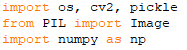
\includegraphics[width=0.4\linewidth]{images/fr_cam7.PNG}
        \caption{Import library}
    \end{figure}

    - Baris ke-1 dan 2 untuk mengambil dataset dengan join direktori tempat kumpulan dataset

    Baris ke -3 untuk memasukan algoritma face detection

    Baris ke-4 untuk proses deteksi wajah dengan algoritma LBPH
    \begin{figure}[h!]
        \centering
        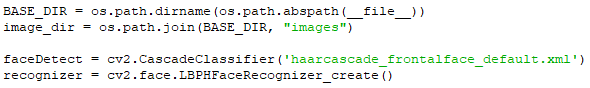
\includegraphics[width=0.9\linewidth]{images/fr_cam8.PNG}
        \caption{Pengambilan dataset }
    \end{figure}

    - Pembuatan variabel array untuk data id dan label gambar
    \begin{figure}[h!]
        \centering
        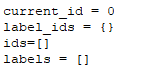
\includegraphics[width=0.3\linewidth]{images/fr_cam9.PNG}
        \caption{Variabel }
    \end{figure}

    \newpage
    - Menelusuri seluruh folder dan mencari gambar, file yang diakhiri 
    dengan jpg. Menggunakan root, untuk menemukan nama folder file dan menyimpannya dalam variabel label. 
    Nama orang yang akan ditampilkan di layar akan menjadi labelnya.
    \begin{figure}[h!]
        \centering
        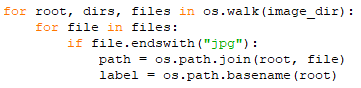
\includegraphics[width=0.7\linewidth]{images/fr_cam10.PNG}
        \caption{Menelusuri folder dataset }
    \end{figure}

    - Proses mengubah gambah menjadi array numpy dan melakukan training data. Untuk mengambil gambar menggunakan library 
    \textbf{Image} Pillow pada python kemudian gambar yang diambilakan dikonversi kedalan grayscale, lalu diubah ke dalam bentur array numpy. 
    Hal ini dilakukan untuk memberikan label terhadap id tertentu. selanjutnya akan dilakukan deteksi wajah menggunakan algoritma \textbf{cascade}
    \begin{figure}[h!]
        \centering
        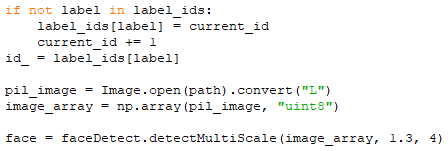
\includegraphics[width=0.8\linewidth]{images/fr_cam11.PNG}
        \caption{Menelusuri folder dataset dan konversi gambar}
    \end{figure}

    - Mengisi bingkai deteksi dengan nama label sesuai kecocokannya
    \begin{figure}[h!]
        \centering
        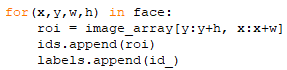
\includegraphics[width=0.5\linewidth]{images/fr_cam12.PNG}
        \caption{Melampirkan nama}
    \end{figure}
    \newpage
    - Menyimpan hasil training data pada file face-trainner.yml
    \begin{figure}[h!]
        \centering
        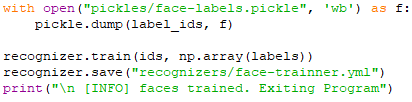
\includegraphics[width=0.7\linewidth]{images/fr_cam13.PNG}
        \caption{Simpan hasil training}
    \end{figure}

    - Keseluruhan program training data
    \begin{figure}[h!]
        \centering
        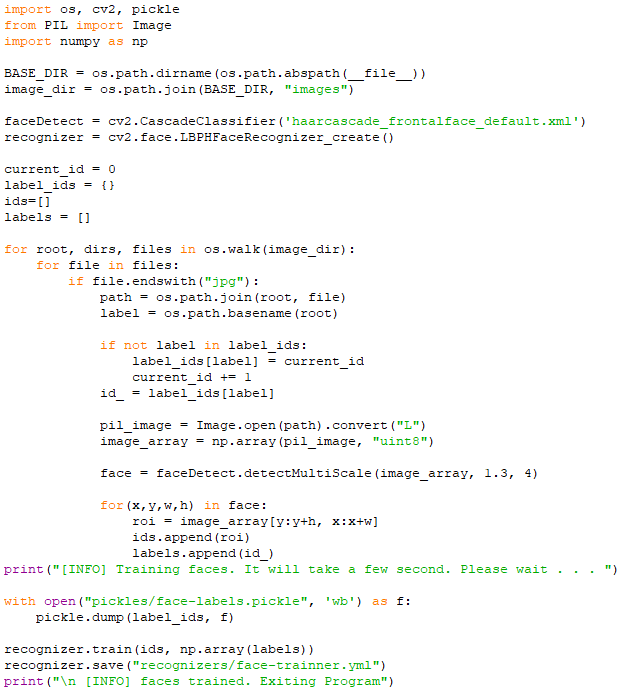
\includegraphics[width=1\linewidth]{images/fr_cam14.PNG}
        \caption{Program training}
    \end{figure}
    \item Proses pengenalan wajah
    
    - Import Library
    \begin{figure}[h!]
        \centering
        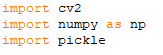
\includegraphics[width=0.4\linewidth]{images/fr_cam15.PNG}
        \caption{Import library}
    \end{figure}

    - Menggunakan algoritma LBPH untuk pengenalan wajah, dengan membaca model file hasil 
    data training sebelumnya. Dan penggunaan library \textbf{pickle} untuk mengambil label nama sesuai id
    \begin{figure}[h!]
        \centering
        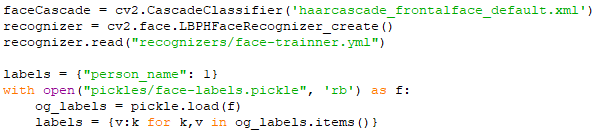
\includegraphics[width=1\linewidth]{images/fr_cam16.PNG}
        \caption{Model trained}
    \end{figure}

    - Pengaturan kamera, pengubahan warna citra menjadi grayscale untuk pencocokan dengan train dataset
    \begin{figure}[h!]
        \centering
        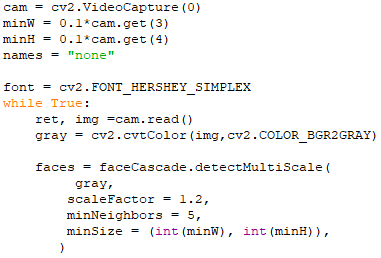
\includegraphics[width=0.65\linewidth]{images/fr_cam17.PNG}
        \caption{Pengaturan kamera}
    \end{figure}
\newpage
    - Proses prediksi untuk pencocokan inputan wajah pada kamera dengan train dataset. 
    Dengan menampilkan label nama sesuai id dan persentase kecocokan.
    \begin{figure}[h!]
        \centering
        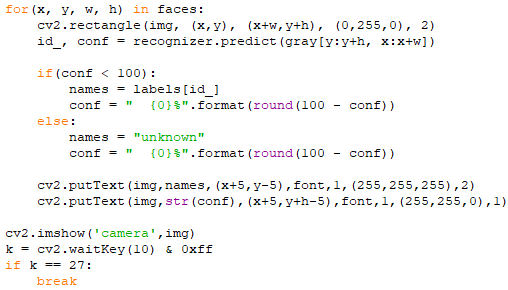
\includegraphics[width=0.8\linewidth]{images/fr_cam18.PNG}
        \caption{Import library}
    \end{figure}

    - Hasil
    \begin{figure}[h!]
        \centering
        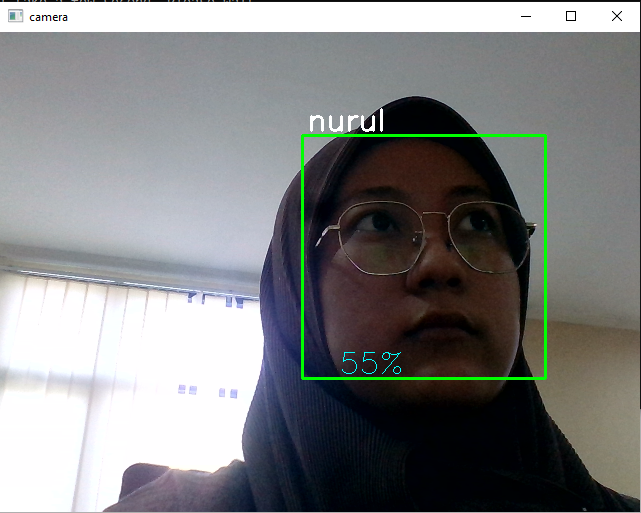
\includegraphics[width=0.8\linewidth]{images/fr_cam_30cm.PNG}
        \caption{Hasil face recognition jarak sekitar 30 cm dengan kamera}
    \end{figure}
    \newpage
    \begin{figure}[h!]
        \centering
        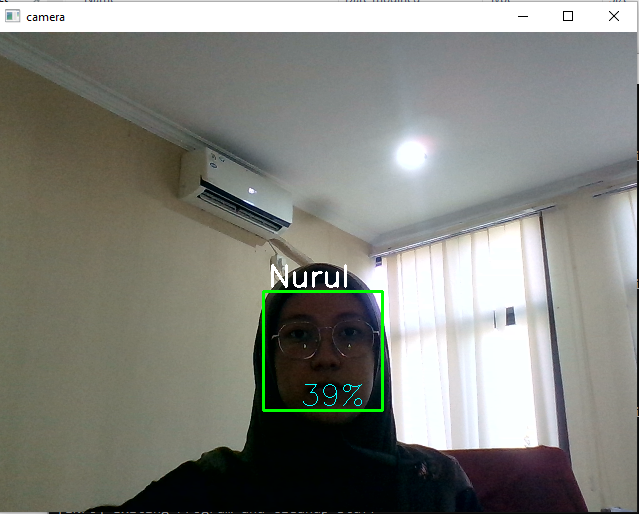
\includegraphics[width=0.8\linewidth]{images/fr_hasil1_1m.PNG}
        \caption{Hasil face recognition jarak sekitar 1 meter dengan kamera}
    \end{figure}
\end{enumerate}